% ================================================================
% SECTION 2: ARCHITECTURE OVERVIEW
% ================================================================
\section{Architecture Overview}
\label{sec:architecture}

\bionetflux{} is organised as a single Python package \code{bionetflux} installed from \code{src/bionetflux/}.  The package is divided into six sub-packages plus a top-level orchestration module.

\subsection{Package Layout}

\begin{center}
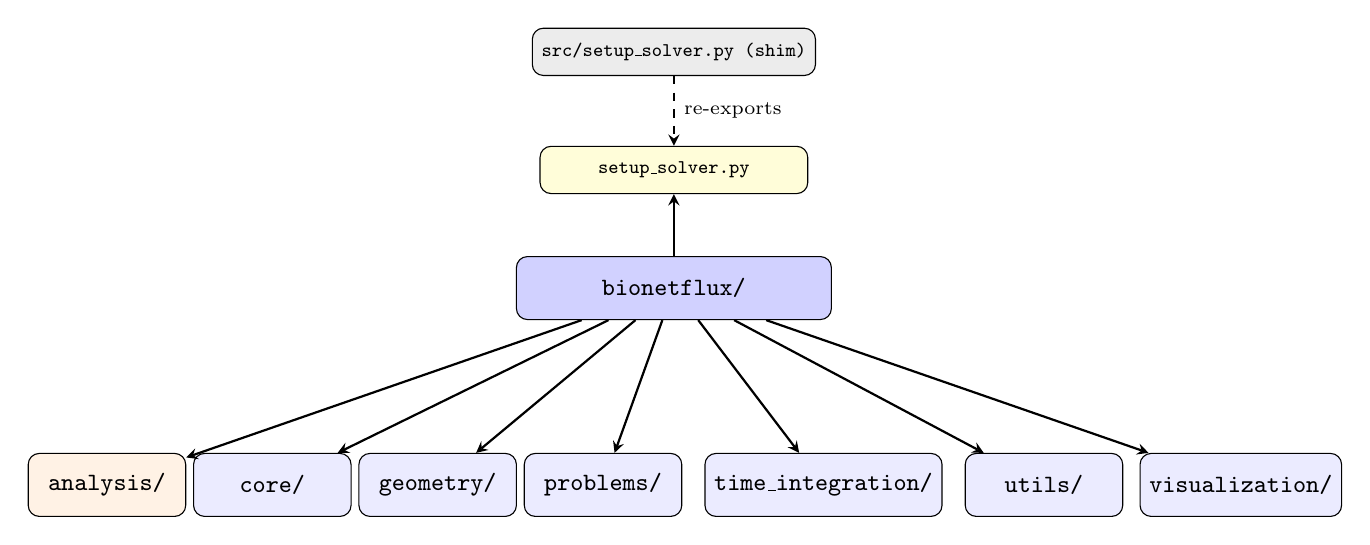
\begin{tikzpicture}[
    pkg/.style={draw, rounded corners, fill=blue!8, minimum width=2.0cm, minimum height=0.8cm, font=\ttfamily\small},
    mod/.style={draw, rounded corners, fill=green!8, minimum width=2.8cm, minimum height=0.6cm, font=\ttfamily\scriptsize},
    arr/.style={->, thick, >=stealth},
    level 1/.style={sibling distance=3.6cm},
]

% Root
\node[pkg, fill=blue!18, minimum width=4cm] (root) at (0,0) {bionetflux/};

% Sub-packages row
\node[pkg] (core)    at (-5.1, -2.5) {core/};
\node[pkg] (geom)    at (-3.0,-2.5) {geometry/};
\node[pkg] (probs)   at (-0.9,  -2.5) {problems/};
\node[pkg] (ti)      at (1.9,-2.5) {time\_integration/};
\node[pkg] (utils)   at (4.7,  -2.5) {utils/};
\node[pkg] (vis)     at (7.2,-2.5) {visualization/};

% analysis
\node[pkg, fill=orange!10] (anal) at (-7.2,-2.5) {analysis/};

% Top-level module
\node[mod, fill=yellow!15, minimum width=3.4cm] (setup) at (0, 1.5) {setup\_solver.py};

% Shim
\node[mod, fill=gray!15, minimum width=3.4cm] (shim) at (0, 3) {src/setup\_solver.py (shim)};

% Edges
\draw[arr] (root) -- (core);
\draw[arr] (root) -- (geom);
\draw[arr] (root) -- (probs);
\draw[arr] (root) -- (ti);
\draw[arr] (root) -- (utils);
\draw[arr] (root) -- (vis);
\draw[arr] (root) -- (anal);
\draw[arr] (root) -- (setup);
\draw[arr, dashed] (shim) -- node[right, font=\scriptsize]{re-exports} (setup);

\end{tikzpicture}
\end{center}

\begin{longtable}{lp{10cm}}
\toprule
\textbf{Sub-package} & \textbf{Contents} \\
\midrule
\code{core/} & Problem base class, Discretization, Constraints, BulkData, DomainData, BulkDataManager, GlobalAssembler, StaticCondensation (base, Keller-Segel, OoC, factory), FluxJump, BoundaryOverride, MinimalErrorEvaluator \\
\code{geometry/} & DomainGeometry, DomainInfo, ConnectionInfo, built-in geometry builders, maze data CSV files \\
\code{problems/} & Keller-Segel and Organ-on-Chip problem modules, config managers, custom problem template, test problems \\
\code{time\_integration/} & TimeStepper, AdaptiveTimeStepper, TimeStepResult, NewtonSolver, NewtonResult \\
\code{utils/} & ElementaryMatrices (sympy-based), BaseConfigManager and FunctionResolver (TOML config), mesh\_mapping \\
\code{visualization/} & LeanMatplotlibPlotter --- 2D curves, 3D flat, bird's eye, comparison, and geometry index plots \\
\code{analysis/} & ErrorEvaluator --- trace/bulk error computation, convergence rates, error reports \\
\bottomrule
\end{longtable}

\noindent The backward-compatible shim \code{src/setup\_solver.py} re-exports \code{SolverSetup}, \code{quick\_setup}, and \code{create\_solver\_setup} so that existing scripts using \code{from setup\_solver import quick\_setup} continue to work.

\subsection{Data Flow Pipeline}

The main computational pipeline follows this sequence:

\begin{center}
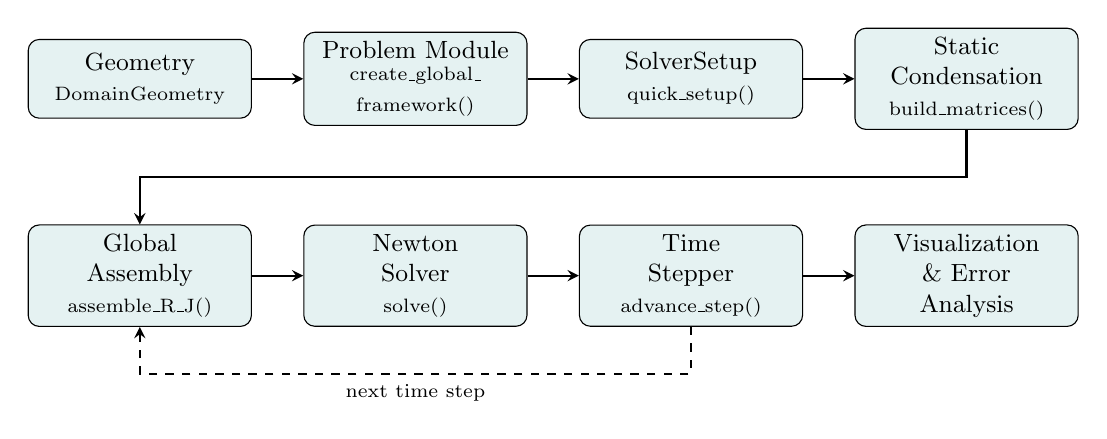
\begin{tikzpicture}[
    box/.style={draw, rounded corners, fill=teal!10, minimum width=2.8cm, minimum height=1.0cm, text width=2.6cm, align=center, font=\small},
    arr/.style={->, thick, >=stealth},
]

\node[box] (geom) at (0,0) {Geometry\\{\scriptsize DomainGeometry}};
\node[box] (prob) at (3.5,0) {Problem Module\\{\scriptsize create\_global\_\\framework()}};
\node[box] (setup) at (7,0) {SolverSetup\\{\scriptsize quick\_setup()}};
\node[box] (sc) at (10.5,0) {Static\\Condensation\\{\scriptsize build\_matrices()}};

\node[box] (ga) at (0,-2.5) {Global\\Assembly\\{\scriptsize assemble\_R\_J()}};
\node[box] (newton) at (3.5,-2.5) {Newton\\Solver\\{\scriptsize solve()}};
\node[box] (ts) at (7,-2.5) {Time\\Stepper\\{\scriptsize advance\_step()}};
\node[box] (vis) at (10.5,-2.5) {Visualization\\\& Error\\Analysis};

\draw[arr] (geom) -- (prob);
\draw[arr] (prob) -- (setup);
\draw[arr] (setup) -- (sc);
\draw[arr] (sc) |- ++(0,-1.25) -| (ga);
\draw[arr] (ga) -- (newton);
\draw[arr] (newton) -- (ts);
\draw[arr] (ts) -- (vis);

% Feedback loop
\draw[arr, dashed] (ts.south) -- ++(0,-0.6) -| node[below, font=\scriptsize, pos=0.25]{next time step} (ga.south);

\end{tikzpicture}
\end{center}

\subsection{Key Design Patterns}

\begin{designbox}
\textbf{Factory Registration.}  \code{StaticCondensationFactory} maintains a dictionary mapping problem-type strings (\code{"keller\_segel"}, \code{"organ\_on\_chip"}) to concrete \code{StaticCondensationBase} sub-classes.  New problem types are added via \code{register\_implementation(type\_str, class)}.
\end{designbox}

\begin{designbox}
\textbf{Lazy Cached Properties.}  \code{SolverSetup} delays the creation of expensive objects --- \code{elementary\_matrices}, \code{static\_condensations}, \code{global\_assembler}, \code{bulk\_data\_manager} --- until first access.  This avoids unnecessary computation when only a subset of components is needed.
\end{designbox}

\begin{designbox}
\textbf{Dynamic Module Import.}  Problem modules are loaded at run-time via \code{importlib.import\_module(problem\_module)}.  Every problem module must expose a function \code{create\_global\_framework(geometry=None, config\_file=None)} that returns a 4-tuple \code{(problems, global\_discretization, constraint\_manager, problem\_name)}.
\end{designbox}

\begin{designbox}
\textbf{TOML Configuration with Function Resolution.}  Physical parameters, initial/boundary conditions, and source terms can be specified in TOML files.  The \code{FunctionResolver} maps string names (e.g., \code{"traveling\_wave\_u"}, \code{"zeros"}) to Python callables and can also parse SymPy string expressions (e.g., \code{"2.5 + 0.0*s"}).
\end{designbox}
